\documentclass[UTF8,a4paper]{paper}
\usepackage{ctex}
\usepackage{multicol}
\usepackage{amsmath}
\usepackage{graphicx}
\usepackage{wrapfig}
\usepackage{listings}
\usepackage{float}
\usepackage[colorlinks,linkcolor=blue]{hyperref}
\title{线性系统控制工程2017\\ 课程总结(个人版)}
\author{\\ \\ \\ \\ \\ \\ \\ \\ 姓名:张蔚桐\\ \\ 学号:2015011493\\ \\  
小组名或组号: MC5-屹立不倒\\ \\ 指导教师:赵明国\\ }
\begin {document}
\maketitle\clearpage
\tableofcontents\clearpage
\section{小组概况及本人角色}
请介绍本人所在小组的名称,同组成员名单,本人在小组项目中的分工。根据所做工作的性质不同,本人承担的分工可以是控制系统需求分析、文献调研、被控对象的建模、控制方案的设计或比较、控制器的设计或实现、闭环系统的性能测试等。
\subsection{所在小组名称:MC5-屹立不倒}
同组成员:贾成君\ 沙星瑜\ 贺秋时。
\subsection{项目背景}
本项目的名称“屹立不倒”是对本项目所做小车的一个简单易懂的解释,本项目最初实现的目标即为使小车“屹立不倒”,经过我们组的努力,也最终使得小车实现了真正意义的“屹立不倒”,同时,采用“屹立不倒”作为我们的项目名称,也表现了我们小组在调试过程中面对各种问题时所展现的持之以恒的精神,在一次次面对难题努力和失败过程中,我们小组屹立不倒,不断努力奋斗,才有机会找到灵感解决之前不能解决的问题,最终终于获得成功的回报。

整个项目的主要是平衡小车的实现,项目背景是最近比较火的二轮自平衡代步工具segway,这款产品在载人的情况下能够保持站立状态,并且随着操纵者重心的移动而前进后退、左转右转。我们的自平衡小车实际是segway的简化版,是其功能的核心部分。

通过对小车的调试实现设计的要求,我们复习领会了控制理论等方面的很多理论知识并将理论知识应用于实践中,了解到了实际工程和理论分析,仿真建模之间的联系和差别。培养了自己的动手能力和工程思想。

具体来说,本项目设计希望利用线性控制系统和自动控制原理两门课程学习的理论知识,设计一个能够自平衡直立的小车,同时希望完成一些诸如原地匀速旋转,匀速运动,向指定目标点运动等附加要求。就项目的最后实现功能来看,我们已经出色的完成了所有既定的要求,甚至在一些性能上远远高出我们开始的预期。目前小车可以实现长期的相当稳定的直立保持,比较快速的完成位置转移和原地旋转的要求。项目成功完成。
\subsection{本人在小组项目中的分工}
主要负责:建模、需求分析、系统性能评价测试、GitHub整理
协助工作:实际小车控制方案设计、仿真控制方案设计、PPT设计、陀螺仪温漂抑制

本人主要完成了对整个系统的建模,包括首先完成了用户需求的分析,确定了直立稳态,匀速前进,指定位置前进和匀速旋转等需求之间的关系和整体的逻辑。使用牛顿力学方法和JMJ方法进行了系统建模分析。最后完成了整体系统性能的评价测试。在整个项目进行的过程中,我对代码托管仓库GitHub进行了及时的整理,方便了后续的开发和工作。

同时,我协助了三位学长完成了实际小车控制方案设计,仿真控制方案的设计,PPT的设计和陀螺仪的温漂控制等工作。提出了一些可行的设计方案。

由于大二年级如电机拖动和运动控制等课程还没有开始学习,在参与对电机的调试过程中自学了不少东西,也在学长的帮助之下相关的知识有了一部分的了解。

\clearpage\section{本人所做的工作}
应该详细描述所承担的研究工作中的研究对象、研究目标(需要解决的问题)、采用的研究方法、取得的结果。此部分报告的重点内容,应尽量详细(参考字数5000字)。

\subsection{需求分析工作}
首先我完成了需求分析的工作,参考了老师的要求,除了原地直立的基本要求,我们设计了上坡下坡,原地旋转,前进后退等多个要求。

经过细致的分析我们发现,从直觉上可以看出,上坡下坡感觉上可以利用轮子对地面的摩擦力解决,在坡度不是太大的情况下不需要作为一个独立的问题研究。坡度比较大的情况下,我们将采用进一步的建模进行分析是否可行,留待之后说明。

之后我们研究了原地旋转的开发需求,从牛顿力学我们知道,小车的行为总可以分解为一个绕轴的旋转和平动两个运动的合成,我们认为旋转对控制小车的平衡没有影响,即使存在影响也应当是由角度量守恒导致的在高速旋转的情况下对向下倾倒的抑制作用,由于小车运动速度达不到这种程度,因此我们可以将这点增益忽略不计。

因此,如果我们希望小车以$\omega$的角速度旋转的话,如果车辆直径为$2r$,我们可以将原控制器得到的速度$v$转换成左轮$v_l=v+r\omega$,右轮$v_r=v-r\omega$。因此这个也不是设计的难点。我们可以在控制器后简单加编程实现。

之后是小车的前进后退的需求,我们认为小车要想前进后退,必然在加速过程中出现倾斜,因此希望直接设计一个能够以任意速度匀速运动的小车是比较有难度的。但是,我们发现让小车稳定在指定位置这一点很容易达到,因此我们考虑设计的过程中为小车设计一个“目标点”,小车向目标点运动,目标点可能随着预期速度的变化而发生变化,因此这个问题也和角度-位置稳定性分析得到了一致的解决。

经过分析我们得到结论,项目的难点在于完成一个对车辆倾斜角度和位置的尽可能小的误差的控制,和之前想法不同的是,我们之前只关心小车是否能直立,而不关心小车直立的位置,现在我们关心小车直立的位置,并以此来对小车的稳定位置和稳定运行(如前进后退)进行控制。实现一个有价值的控制体系。

\subsection{数学建模工作}
为了对小车进行控制,我们需要首先建立Segway小车的物理模型,我们把小车分为车体(B)和轮子(W)两部分;车体上的人简化为摆杆模型,车轮简化为输出转矩的独轮,模型图如图\ref{1}所示。其中涉及的各个量的符号和数值由表\ref{t1}给出。
\begin{table}\centering
\caption{涉及到的常量数值}\label{t1}
\begin{tabular}{|c|c|c|}\hline
参数 & 符号 & 数值和单位 \\ \hline
车体质量 & $m_B$ &$80\mathrm{kg}$ \\ \hline
车体回转半径 & $r_B$ &$0.4\mathrm{m}$\\ \hline
车体转动惯量&$I_B$&$12.8\mathrm{kg\cdot m^2}$\\ \hline
车体质心高度 & $l$ &$1.0\mathrm{m}$\\ \hline
车轮质量 & $m_W$ &$5\mathrm{kg}$\\ \hline
车轮回转半径 & $r_W$ &$0.1\mathrm{m}$\\ \hline
车轮转动惯量&$I_B$&$0.05\mathrm{kg\cdot m^2}$\\ \hline
车轮半径&$R$&$0.254\mathrm{m}$\\ \hline
重力加速度&$g$&$9.8015\mathrm{m/s^2}$ \\ \hline
\end{tabular}\end{table}
\begin{figure}\centering
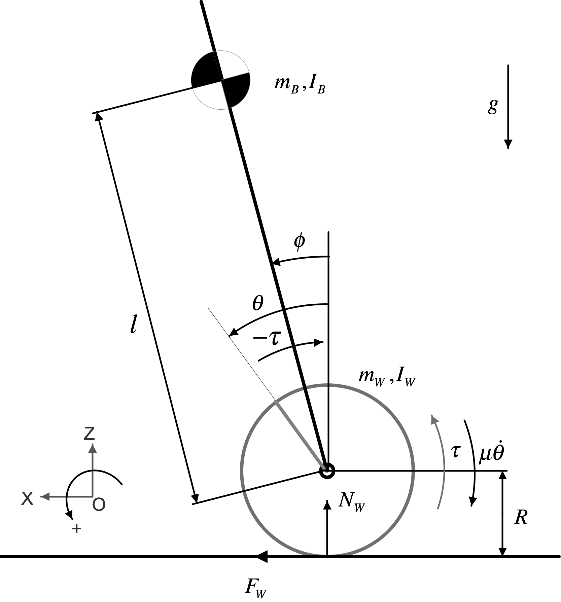
\includegraphics[width=\columnwidth]{1.png}
\caption{小车的理论抽象模型}
\label{1}
\end{figure}

我们采用了JMJ方法和牛顿力学方法进行了建模,通过两种方法的相互印证和对比,我们也对两种方法的优势和劣势有了进一步的了解。
\subsubsection{JMJ方法建模}
首先我们描述JMJ方法。从图\ref{1}我们可以看出,$F,F_W,N_W$都是不做功的力,在建模中可以忽略,因此我们得到了如下的广义坐标和广义力的表达式:
\begin{equation}
q = \begin{pmatrix} \theta & \phi \end{pmatrix}^\mathrm{T}
\end{equation}
\begin{equation}
x(q) = \begin{pmatrix}R\theta&0&\theta&R\theta+l\sin(\phi)& l\cos(\phi)& \phi \end{pmatrix}^\mathrm{T}
\end{equation}
\begin{equation}
F^\mathrm{a} = \begin{pmatrix} 0&-m_wg&\tau-\mu\dot{\theta}&0&-m_Bg&0\end{pmatrix}^\mathrm{T}
\end{equation}
\begin{equation}
M = diag\begin{pmatrix}m_W&m_W&I_W&m_B&m_B&I_B\end{pmatrix}\end{equation}
并进一步得到状态空间方程并进行线性化使得$\cos\phi=1,\sin\phi=\phi,\dot{\phi}^2=0$得到线性化后的状态空间模型:
\begin{equation}
x = \begin{pmatrix}\theta&\phi&\dot{\theta}&\dot{\phi}\end{pmatrix}^\mathrm{T}\end{equation}
\begin{equation}
A = \begin{pmatrix}
0&0&1&0\\0&0&0&1\\
0&-\frac{Rgl^2m_B^2}{P}&-\frac{\mu m_Bl^2+\mu I_B}{P}&0\\
0&\frac{lm_B(I_Wg+m_BR^2g+m_WR^2g)}{P}&\frac{\mu Rlm_B}{P}&0\end{pmatrix}\end{equation}
\begin{equation}
B = \begin{pmatrix}0&0&\frac{m_Bl^2+I_B}{P}&-\frac{Rlm_B}{P}\end{pmatrix}^\mathrm{T}\end{equation}
\begin{equation}
C = \begin{pmatrix} 1&0&0&0\\0&1&0&0\end{pmatrix}\end{equation}
\begin{equation}D = \begin{pmatrix}0&0\end{pmatrix}^\mathrm{T}\end{equation}
其中参量$P = (I_W+m_WR^2+m_BR^2)(I_B+m_Bl^2-m_BR)^2$,带入表\ref{t1}中的具体数值得到$A$和$B$矩阵为:
\begin{equation}A=\begin{pmatrix}
0&0&1&0\\0&0&0&1\\0&-158.3&-0.07377&0\\0&43.12&0.01615&0\end{pmatrix}\end{equation}
\begin{equation}B=\begin{pmatrix}
0&0&0.9221&-0.2019\end{pmatrix}^\mathrm{T}\end{equation}
使用JMJ方法,我们得到了传递函数。
\subsubsection{牛顿力学分析}
先对轮子进行受力分析,考虑到轮子是纯滚动状态,得到
\begin{equation}
I_w\ddot{\theta}=\tau-F_wR-\mu\dot{\theta}
\label{1}
\end{equation}
\begin{equation}
m_wR\ddot{\theta}=-F_x+F_w
\label{2}
\end{equation}
式中考虑到了$x=R\theta$的纯滚条件,同时认为轮胎的摩擦系数满足纯滚条件

下一步研究杆的运动状态,角量上有
\begin{equation}
I_B\ddot{\phi}=F_yl\mathrm{sin}\phi-F_xl\mathrm{cos}\phi
\label{3}
\end{equation}
平动方程
\begin{equation}
F_x=m_B\ddot{x}
\label{4}
\end{equation}
\begin{equation}
m_B\mathrm{g}-F_y=m_B\ddot{y}
\label{5}
\end{equation}
运动学关联我们有
\begin{equation}
x-l\mathrm{sin}\phi=R\theta
\label{6}
\end{equation}
\begin{equation}
y=l\mathrm{cos}\phi
\label{7}
\end{equation}
下面开始解方程

从(\ref{1}),(\ref{2})得到
\begin{equation}
I_w\ddot{\theta}+F_xR+m_wR^2\ddot{\theta}=\tau-\mu\dot{\theta}
\label{8}
\end{equation}
结合(\ref{4})得到
\begin{equation}
(I_w+m_wR^2)\ddot{\theta}+m_BR\ddot{x}+\mu\dot{\theta}=\tau
\label{9}
\end{equation}
对(\ref{6})求导得到
\begin{equation}
\ddot{x}-l\mathrm{cos}\phi\ddot{\phi}+l\mathrm{sin}\phi\dot{\phi}^2=R\ddot{\theta}
\label{10}
\end{equation}
带入(\ref{9})得到
\begin{equation}
(I_w+m_wR^2+m_BR^2)\ddot{\theta}+m_BRl(\mathrm{cos}\phi\ddot{\phi}-\mathrm{sin}\phi\dot{\phi}^2)+\mu\dot{\theta}=\tau
\label{11}
\end{equation}
联立(\ref{3}),(\ref{4}),(\ref{5})得到
\begin{equation}
I_B\ddot{\phi}=(m_B\mathrm{g}-m_B\ddot{y})l\mathrm{sin}\phi-m_B\ddot{x}l\mathrm{cos}\phi
\label{12}
\end{equation}
对(\ref{7})式求导得到
\begin{equation}
\ddot{y}=-l\mathrm{cos}\phi\dot{\phi}^2-l\mathrm{sin}\phi\ddot{\phi}
\label{13}
\end{equation}
联立(\ref{10}),(\ref{12}),(\ref{13})得到
\begin{equation}
I_B\ddot{\phi}=(m_B\mathrm{g}+m_Bl(\mathrm{cos}\phi\dot{\phi}^2+\mathrm{sin}\phi\ddot{\phi}))l\mathrm{sin}\phi-m_B(R\ddot{\theta}+l\mathrm{cos}\phi\ddot{\phi}-l\mathrm{sin}\phi\dot{\phi}^2)l\mathrm{cos}\phi
\label{14}
\end{equation}
稍作整理得到
\begin{equation}
I_B\ddot{\phi}=m_B\mathrm{g}l\mathrm{sin}\phi + m_Bl^2\mathrm{sin}(2\phi) \dot{\phi}^2-m_Bl^2 \mathrm{cos}(2\phi)\ddot{\phi}-m_BRl\mathrm{cos}\phi\ddot{\theta}
\label{15}
\end{equation}
联立(\ref{11}),(\ref{15})并进行线性化得到
\begin{equation}
(I_w+m_wR^2+m_BR^2)\ddot{\theta}+m_BRl\ddot{\phi}+\mu\dot{\theta}=\tau
\label{16}
\end{equation}
\begin{equation}
I_B\ddot{\phi}=m_B\mathrm{g}l\phi-m_Bl^2 \ddot{\phi}-m_BRl\ddot{\theta}
\label{17}
\end{equation}
到这里我们发现和之前JMJ方法得到的结论等价,后面的带入数值计算就省略了。
\subsubsection{斜坡情况的分析}
我们选择牛顿力学对斜坡进行分析来找出他们分不同点,为保持和之前的坐标系一致,我们采用平行于平面和垂直于平面的两个方向作为坐标系建模。假设斜坡倾角为$\alpha$

先对轮子进行受力分析,考虑到轮子是纯滚动状态,取地面顺心作为角速度参考点可以得到
\begin{equation}
(I_w+m_wR^2)\ddot{\theta}=\tau-F_xR-\mu\dot{\theta}+m_w\mathrm{g}R\mathrm{sin}\alpha
\end{equation}

式中考虑到了$x=R\theta$的纯滚条件,同时认为轮胎的摩擦系数满足纯滚条件

下一步研究杆的运动状态,我们取杆和车的连接处作为角动量参考点,这个点所对应的参考系并非是惯性系,非惯性力有力矩作用,表达式为

\begin{equation}
(I_B+m_Bl^2)\ddot{\phi}=m_B\mathrm{g}l\mathrm{sin}(\phi+\alpha)-m_BRl\mathrm{cos}\phi\ddot{\theta}-\tau
\end{equation}

下面考虑杆的平动,可以得到

\begin{equation}
F_x=m_B\ddot{x}
\end{equation}

同时进一步考虑运动学关联,可以得到

\begin{equation}
x-l\mathrm{sin}\phi=R\theta
\end{equation}

求导得到

\begin{equation}
\ddot{x}-l\mathrm{cos}\phi\ddot{\phi}+l\mathrm{sin}\phi\dot{\phi}^2=R\ddot{\theta}
\end{equation}

综合带入方程可以得到
\begin{equation}
(I_w+m_wR^2+m_BR^2)\ddot{\theta}+m_BRl(\mathrm{cos}\phi\ddot{\phi}-\mathrm{sin}\phi\dot{\phi}^2)+\mu\dot{\theta}=\tau+m_w\mathrm{g}R\mathrm{sin}\alpha
\end{equation}
\begin{equation}
(I_B+m_Bl^2)\ddot{\phi}=m_B\mathrm{g}l\mathrm{sin}(\phi+\alpha)-m_BRl\mathrm{cos}\phi\ddot{\theta}-\tau
\end{equation}

下面分析一下这个方程,首先验证正确性,当$\alpha=0$时退化为之前讨论的方程,即

\begin{equation}
(I_w+m_wR^2+m_BR^2)\ddot{\theta}+m_BRl(\mathrm{cos}\phi\ddot{\phi}-\mathrm{sin}\phi\dot{\phi}^2)+\mu\dot{\theta}=\tau
\end{equation}
\begin{equation}
(I_B+m_Bl^2)\ddot{\phi}=m_B\mathrm{g}l\mathrm{sin}\phi-m_BRl\mathrm{cos}\phi\ddot{\theta}-\tau
\end{equation}

其次讨论线性化条件,首先我们应该看到,如果$\phi=0$的话,系统不可能保持平衡,稍加分析我们就可以知道,这里的趋近于0的量应当是$\phi+\alpha$,即车辆实际上车体始终保持着绝对的竖直状态,因此我们记$\phi^*=\phi+\alpha$来进行下一步的线性化工作

线性化得到

\begin{equation}
(I_w+m_wR^2+m_BR^2)\ddot{\theta}+m_BRl\mathrm{cos}\alpha\ddot{\phi^*}+\mu\dot{\theta}=\tau+m_w\mathrm{g}R\mathrm{sin}\alpha
\end{equation}
\begin{equation}
(I_B+m_Bl^2)\ddot{\phi^*}=m_B\mathrm{g}l\phi^*-m_BRl\mathrm{cos}\alpha\ddot{\theta}-\tau
\end{equation}

和之前得到的线性化模型比较得到他们的差别

\begin{equation}
(I_w+m_wR^2+m_BR^2)\ddot{\theta}+m_BRl\ddot{\phi}+\mu\dot{\theta}=\tau
\label{116}
\end{equation}
\begin{equation}
(I_B+m_Bl^2)\ddot{\phi}=m_B\mathrm{g}l\phi-m_BRl\ddot{\theta}-\tau
\label{117}
\end{equation}

利用JMJ方法,我们也能得到相同的结论,但是相比JMJ方法,牛顿方法中的重力的分解更能体现这个问题的本质。

比较斜坡和平面状态下小车的运动方程,首先,部分常量的值发生了一些变化;其次,在对系统进行控制的过程中会加入了恒定的扰动。也就是说,同样的控制策略,如果能够使得小车在平面上稳定运动,并留有比较合适的稳定裕量,小车是可以在斜面上以一个加速度运动的,这个加速度由重力分力给出。同时,我们已经看出小车在水平面上做到位置闭环稳定(就是可以稳定在任何指定的位置上),因此如果我们可以设计小车在水平面上以一个加速度运动,那么我们就也可以用几乎相同的控制原理控制小车在斜面上匀速运动或者保持静止。考虑导致这种相对比较简单的情况的原因,我们认为这和轮轴处可以随意旋转导致车体和斜坡之间解耦有一定的关系。

因此,想要做到小车在斜坡和平面上都比较稳定的运动是有可能的,而且是相对比较容易达到的。其中稳定运动的目标应当是小车车体完全竖直(而不是和平面竖直)

当然,还需要考虑斜面的曲率和倾角不能过于极端导致小车出现了不可控的滑动的情况。这种情况相对比较极端,在我们的项目中也没有这种极端情况下的需求,在这种情况下,摩擦力可能变为滑动摩擦力,同时重力力矩也可能使小车出现翻倒的情况,具体的情况就比较复杂了,这里就不继续说明了。
\subsubsection{小结}
从两个分析方式我们可以看到,分析力学JMJ方法忽略了很多无关的变量,利用分析力学方法,使得整个分析过程变得程序化,在利用MATLAB进行辅助计算时相对比较简单。牛顿力学方法需要细致讨论所有的力的贡献,需要更多的“专家经验”,计算上的技巧性也比较大,得到的结果也相对比较全面。后续的工程也证明,JMJ方法虽然比较简单,但是忽略了一些比较重要的存在,例如牛顿方法中我们可以明确的看出摩擦力和支持力两个约束力的关系,得到平面最小摩擦系数的表达式,而JMJ方法忽略了这些问题。实际项目中我们也可以看出,在光滑的地面上,小车的表现相对在毛毯等粗糙的地面上相对差一点。如果想从理论上彻底的分析这个问题,就必须要研究约束力了。同时从对斜坡的分析我们也可以看到,牛顿力学方法可以更好的分析问题的本质,而JMJ方法可以更快的得到需要的结论。

同时,关于斜面的分析我们可以看出,只要控制系统设计的稳定并且留有一定的裕量,小车是可以在斜面上保持想要的运动效果的,尤其是对于坡度较小的斜面而言,斜面的存在可以忽略不计或认为是一种水平表面上存在的扰动,当做噪声处理。当然,当斜面坡度逐渐变大时,相关的控制难度就变大了。设计的控制系统也是存在着一定的试用范围的。

总的来说,两种方法各有优劣,就本项目设计而言,JMJ方法和后续的工程的耦合性比较好。牛顿力学方法可以作为一个分析问题,找到问题根源的一种分析手段和工具。
\subsubsection{后续工作和仿真方案设计}
同时我们可以看出,系统状态矩阵能观能控,想要做到小车在斜坡和平面上都比较稳定的运动是有可能的,而且是相对比较容易达到的。其中稳定运动的目标应当是小车车体完全竖直(而不是和平面竖直)。当然,还需要考虑斜面的曲率和倾角不能过于极端导致小车出现了不可控的滑动的情况。这一点由后续控制策略的同学出色的完成了相关的设计。我协助完成了一些仿真方案的设计工作。

\subsection{系统性能的评价和测试}
在小组完成了小车的搭建之后,我参与了系统性能的评价和测试工作,和小组成员一起完成了对小车整体性能的评价和测试,提出了一些可行的改进建议。

对于我们小组,在调试过程中遇到的最大困难是陀螺仪的零点误差等问题。陀螺仪由于陀螺仪输出的角速度值就带有不少温漂和毛刺,导致积分之后输出的角度差别更加明显,因此我们小组采用了几个步骤和多种方法来尽可能的减少输出的误差。

首先对于陀螺仪输出的角速度毛刺(高频),我们采用了均值滤波和巴特沃斯滤波,融合滤波等几种方式来处理,这里将几种滤波方式的原理和效果简述如下。

均值滤波是取连续的五个时间点上陀螺仪的值作为输出,经过观察我们发现这种方式出现的波形整体比较平滑,当时也存在着一些问题。首先,均值滤波的响应相对较慢,因为他是一个延时的系统。而均值滤波也无法解决低频偏置带来的积分导致角度巨大误差的问题,我们不采用均值滤波。

融合滤波是一种综合了陀螺仪信息和加速度计信息的滤波方法。这种滤波方法是考虑到:陀螺仪易受震动、温度和不稳定力矩等影响,产生漂移误差,计算小车姿态倾角时由于积分作用其测量误差会越来越大;而加速度计测量的是线性运动,输出加速度信号,速度变化越快,输出值越大,对myRio的z轴加速度计输出值通过三角变换可得到加速度计与重力方向的夹角。

然而,虽然加速度计没有累计误差,但是由于加速度计测量加速度的原理是根据其在myRio参考系中所受惯性力大小而推测加速度的,在动态情况下无法获取稳定的加速度值,易受震动干扰而在静态情况下的加速度值上叠加较大的噪声。对这个特性最直观的理解就是即使小车实现了直立,由于直立的本质是在平衡位置做很小幅度的振荡,此时加速度计给出的加速度值在0的附近做幅度较大的振荡,而不是基本稳定在0。同时我们发现myRIO上加速度计过于敏感,桌面受到震动时也会出现明显的抖动。

因此,仅单独使用陀螺仪或者加速度计对小车姿态进行测量, 很难保证测量结果的精确性和可靠性,因此我们最后放弃了这个方案。

巴特沃斯滤波采取了LabView中给出的巴特沃斯滤波器进行实现,经过调整参数我们发现,巴特沃斯滤波相比之前几个延时性能提升,但是仍然无法解除角速度低频偏置导致的对角速度积分之后得到角度的偏移问题,因此我们一方面采取巴特沃斯滤波器得到当前的角速度值,另一方面我们在积分的过程中试图减去低频偏置修正角速度得到比较准确的角度,而偏置的具体计算方法,我们尝试了如下几种方式。

第一种尝试是设置一个静态的偏置,使得积分之前先减去偏置,调试偏置的过程完全靠人工来调试,然而经过了很长时间的调试,我发现不论如何都不能完全抵消相关的偏置问题,这一方面和测试偏置值的精度不足,同时也和陀螺仪温度发生变化,陀螺仪温度偏置发生变化有关,我们可以看到,这种低频的温漂显然不可能是直流信号,它必然随着温度的波动和工作状态的波动有一些变化,因此试图设计一个直流信号减除偏置是没有意义的,基本没有实用价值。

第二种尝试是在开机之前先让小车静止20秒,陀螺仪完成一个积分过程测量实时的积分值作为之后的偏置减去,这种方式相对于之前的方式可能更能适应更多的环境温度,偏置可以随着温度自行调整。但是缺点是一方面静止20秒这个设定缺乏人性化,需要人工给出一个相当稳定的直立状态,否则短短20秒积分得到的偏置必然存在着相当大的误差。另一方面积分20秒不一定能得到准确的偏置,同时也不能克服在运行过程中的环境温度的变化的影响,具体的问题和第一点相同,唯一相比于第一点有所改进的是,这种方式能够适应不同的初始温度,虽然对于温度波动仍然无能为力。

最后的一个想法是由我的队友提出来的,经过测试发现,检测电机转速的码盘精度要远远高于陀螺仪的精度,因此我们设计在普通的反馈系统中加入速度-角度闭环,简言之,就是希望电机尽可能的少提供加速度,经过测试我们发现,这种方式能够在给出一定的偏置之后,通过反馈消除之后陀螺仪温漂的影响,从根本上解决了这种问题,实现了小车直立的可持久化。另外,我们也尝试了完全不加偏置,经过很长距离的辅助小车矫正之后,小车也能够完成自行的矫正工作。

\subsection{GitHub整理和PPT设计协助}
在整个工程进展过程中,我们提出了很多的方案,也进行了团队合作处理不同的问题,因此团队合作的调度就成了一个重要的工作。我们采用了通用的代码托管仓库GitHub完成了这类工作,整个项目托管在
\url{https://github.com/ZeroWeight/LC/tree/master/Project}中。本人除了自己的工作外,完成了整个仓库的日常维护工作,维护了仓库的合理的文件结构,解决了很多团队合作开发中出现的文件版本的问题,使得整个开发和合作变得十分顺利。

整个团队的代码提交情况如\url{https://github.com/ZeroWeight/LC/graphs/contributors}所示,也可见\url{https://github.com/ZeroWeight/LC/graphs/commit-activity}

同时我也协助队友完成了有关PPT设计等工作。

\clearpage\section{本人课程学习总结}
学习本课程的收获,体会,以及对课程改进的建议。(参考字数400字)

回顾这门课的学习历程,付出了很多,收获也很多。

首先我要感谢我的三位学长队友的帮助和付出,大二年级选修这门课程,学习的压力比较大,尽管已经自学完成了自控I相关课程,理论部分的学习也没有过于吃力,但是开始做项目时才发现自己还有很多知识没有学习。我也深刻意识到了不论是科研项目还是工程都是很多知识有机组合在一起才能得到解决的,仅仅懂得控制理论的知识,让我在面对电机控制,陀螺仪控制的问题过程中显得心有余而力不足,甚至不了解利用PWM控制电机转速的原理,是我的三个队友帮助我解决了这方面的问题,在这个过程中,我也对后续课程和这些知识有了一个感性的上的了解,了解了这些知识的巨大的实用价值。

其次这门课程也是我第一次作为团队中的一员来参加项目的开发,整个项目开发的过程让我体会到了团队合作的力量,也让我意识到了GitHub等代码托管,团队协作的重要性,为之后的团队项目做好了铺垫。

另外,通过实际工程的实践,我也对控制理论有了更深入的认识,我意识到了理论和实践的巨差差距,在进行建模分析的过程中,我曾经认为整个项目比较简单,只需要实现一个PID控制即可,但是实际项目过程中从对检测装置的矫正,到对执行机构的稳定运行,都花费了我们不少的精力,也深刻的体会到了“工程”二字的重要意义,很多知识都不是书本上面能够给我们的,需要很多实际操作的经验,例如PID调参,整个的流程和我们自控里面学过的矫正有相似点但绝不相同,从实际工程中获得知识,这也是我从这门课程中学到的。也感谢老师和助教让我明白了这些差别,增长了不少工程经验。

最后谈到课程建议,我认为由于年级之间的交流,单就一个项目而言,项目的整体难度也会逐渐变低,这是一个不可避免的趋势。从另一方面来讲,作为校级挑战性课程,线控的挑战项目本身也应当更快地跟上科技发展的步伐,因此我建议课程的项目应当每年有所改进创新,一方面允许学弟们向学长请教经验,一方面也鼓励同学们自己动手,自己提出新想法,新设计。
\end{document}